\xchapter{Reconhecimento de software acadêmico de análise estática}
{}\label{estudo2}

\begin{comment}

% macros LaTeX com os resultados encontrados no estudo
% dados do estudo1
\newcommand{\SoftwareCount}{60}
\newcommand{\SoftwareUrlNotAvailableCount}{15}
\newcommand{\SoftwareUrlAvailableCount}{45}
\newcommand{\SoftwareDownloadNotAvailableCount}{24}
\newcommand{\SoftwareDownloadAvailableCount}{36}
% dados do estudo2
\newcommand{\SearchACMCount}{438}
\newcommand{\SearchIEEECount}{459}
\newcommand{\SearchCount}{897}
\newcommand{\SearchUniqueCount}{806}
\newcommand{\ScreeningCount}{429}
\newcommand{\ScreeningUniqueCount}{416}
\newcommand{\CiteCount}{199}
\newcommand{\UseCount}{124}
\newcommand{\ContributeCount}{106}
\newcommand{\SearchUniqueMean}{13.4}
\newcommand{\ScreeningMean}{7.2}
\newcommand{\ScreeningUniqueMean}{6.9}
\newcommand{\MentionsStudyUm}{60}
\newcommand{\MentionsStudyDois}{47}
\newcommand{\SoftwareNotMentionedCount}{13}
\newcommand{\ContributeStudyDoisCount}{43}
\newcommand{\ContributeStudyDoisSoftware}{17}
% dados do estudo3
\newcommand{\ReleasesCount}{303}
\newcommand{\ReleasesAvailableCount}{211}
\newcommand{\ReleasesMetricsCount}{206}
\newcommand{\ProjectsWithReleasesCount}{35}
\newcommand{\ProjectsAnalizedCount}{24}
\newcommand{\ReleasesYearFirst}{2001}
\newcommand{\ReleasesYearLast}{2017}



Este capítulo apresenta 
um estudo para caracterização de software acadêmico de análise estática,
em termos de 
menções e citações (formais e informais) ao software,
uso do software no contexto de outras pesquisas,
e contribuições ao software acadêmico.

O estudo realizado teve como ponto de partida 
o conjunto de projetos de software identificado 
no estudo sobre publicização do software acadêmico (capítulo~\ref{estudo1}).
Uma revisão da literatura nas bases da ACM e IEEE 
encontrou \SearchUniqueCount \ artigos com menções 
-- COLOCAR -- 
ao software acadêmico de análise estática 
desse conjunto.

A seção \ref{estudo2:introducao} contextualiza o estudo,
a seção \ref{estudo2:fundamentacao} apresenta os conceitos teóricos necessários para compreensão do trabalho,
a seção \ref{estudo2:escopo} descreve o objetivo e apresenta as questões de pesquisa,
a seção \ref{estudo2:planejamento} apresenta um planejamento do estudo,
as seções \ref{estudo2:preparacao} e \ref{estudo2:coleta} apresentam detalhes sobre a preparação e execução da coleta de dados,
as seções \ref{estudo2:analise} e \ref{estudo2:interpretacao} apresentam a análise e interpretação dos dados e
a seção \ref{estudo2:conclusoes} traça as conclusões finais deste estudo.

\end{comment}

Este capítulo apresenta
um estudo de caracterização do reconhecimento de software acadêmico de análise estática.
Com base em informações sobre
citações formais e informais ao software acadêmico de análise estática
extraídas de um conjunto de artigos científicos publicados em periódicos ou conferências,
as relações entre software acadêmico e artigos científicos
são identificadas e classificadas % em níveis de colaboração 
para caracterizar o grau de reconhecimento do software acadêmico.

A seção \ref{estudo2:introducao} contextualiza o estudo
e a seção \ref{estudo2:escopo} apresenta seu objetivo e questões de pesquisa.
A seção \ref{estudo2:planejamento} apresenta o planejamento do estudo, e
as seções \ref{estudo2:preparacao} e \ref{estudo2:coleta} descrevem a preparação e execução da coleta de dados.
As seções \ref{estudo2:analise}, \ref{estudo2:interpretacao} e \ref{estudo2:ameacas}
apresentam a análise de dados, interpretação de resultados e ameaças à validade, respectivamente.
Finalmente, a seção \ref{estudo2:conclusoes} traça as conclusões do estudo.

\section{Motivação} \label{estudo2:introducao} % {{{

Um dos sintomas de 
{\it ``dysfunctional chaotic churn''} \cite{howison2015understanding}
em software acadêmico é a quantidade elevada de projetos 
com características e funcionalidades parecidas, 
e comunidades desconectadas e paralelas.
Neste cenário, alguns projetos de software acadêmico
podem se destacar e obter o \textit{reconhecimento} de seus pares.

A prática científica de citação formal entre publicações, amplamente
adotada e praticada entre cientistas de todas as áreas, não é realidade quando
se trata de artefatos digitais, como dados ou código.
Em geral, software é citado na literatura acadêmica
de maneira informal: em notas de rodapé, seções de agradecimentos, e outras
seções ao longo do texto. Usualmente se faz referência ao nome, ocasionalmente
cita-se o número da versão, e raramente usa-se citação formal.
%E o reconhecimento?

Qualquer um que trabalhe com software acadêmico saberá que o nível de
reconhecimento e retribuição para o software e para quem revisa ou desenvolve o
software não é proporcional a sua importância para a Ciência, o sistema de
recompensa científico é quase que exclusivamente baseado em publicações e,
infelizmente, compartilhar software ainda provê pouco mérito dentro do sistema
de recompensa científico, mesmo que o software seja realmente útil para outros
pesquisadores \cite{goble2014better}.

No entanto, o desenvolvimento de sotware acadêmico é uma atividade que consome recursos
(tempo, dinheiro e atenção) e afeta a conduta da Ciência, tanto no geral como
em campos específicos.
O compartilhamento e colaboração no desenvolvimento destes projetos é vista
neste estudo como uma importante estratégia para lidar com o baixo orçamento
das pesquisas, bem como para mitigar os problemas do limitado tempo dos
cientistas e da alta rotatividade entre os grupos de pesquisa.

Esta estratégia de colaboração se torna especialmente interessante entre as
pesquisas da Engenharia de Software, onde, a princípio os cientistas possuem
acesso ao conhecimento e práticas necessárias para o trabalho colaborativo.
Neste estudo, investigamos como os projetos de software acadêmico
de análise estática são mencionados em publicações nas bases da ACM e IEEE e se
há colaboração entre eles.

% }}}

\section{Fundamentação} \label{estudo2:fundamentacao}

Neste estudo,
o termo \textit{menção} é usado para tratar, genericamente, qualquer ocorrência de
nome de projeto de software acadêmico de análise estática em artigo científico,
incluindo tanto citação formal, quanto informal.
Uma menção pode estar associada ao uso do software no contexto de outras pesquisas,
e até mesmo a contribuições ao projeto de software acadêmico.
Desse modo, uma menção define uma relação entre um artigo científico e 
um software acadêmico.

% }}}

\section{Escopo} \label{estudo2:escopo} % {{{

Esta pesquisa teve como ponto de partida
o conjunto de projetos de software identificado
no estudo sobre publicização do software acadêmico de análise estática (capítulo~\ref{estudo1}).
O objetivo de pesquisa está definido segundo a estrutura GQM \cite{basili1994goal}.

\subsection{Definição do Objetivo}

\begin{description}
  \item{\bf Objeto de estudo.}
    O objeto de estudo são os projetos de software de análise estática
    publicados nas conferências ASE e SCAM, identificados no estudo sobre
    publicização do software acadêmico (capítulo~\ref{estudo1}).
  \item{\bf Propósito.}
    O propósito deste estudo é caracterizar as menções feitas a projetos de
    software acadêmico de análise estática.
  \item{\bf Perspectiva.}
    A perspectiva considerada é a de cientista preocupado com o funcionamento
    do ecossistema de software acadêmico e interessado em saber quais são os
    os projetos de software acadêmico de análise estática mais citados na
    literatura acadêmica.
  \item{\bf Foco de qualidade.}
    O principal aspecto de qualidade estudado é a citabilidade
    \cite{smith2016software} do software acadêmico em termos de número e tipo
    de mençoes.
  \item{\bf Contexto.}
    As menções ao software acadêmico de análise estática devem ser extraídas de
    artigos científicos publicados até 2017, e disponíveis nas bases ACM e
    IEEE.  Adicionalmente, as menções serão classificadas com base no
    reconhecimento dado pelo artigo científico ao software acadêmico mencionado
    (conforme Tabela~\ref{esquema-de-mencao},  seção~\ref{estudo2:coleta}).
\end{description}

\subsection{Sumário da Definição}

Analisar os \textit{projetos de software acadêmico de análise estática publicados nas conferências ASE e SCAM}
com o propósito de \textit{caracterizar menções}
com respeito a \textit{citabilidade do software acadêmico}
na perspectiva de \textit{cientistas}
no contexto de \textit{publicações nas bases ACM e IEEE}.

\subsection{Questões de Pesquisa}

Neste estudo, três questões de pesquisa a respeito dos projetos de
software acadêmico de análise estática serão investigadas:

\newcommand{\EstudoDoisQuestaoUm}{
  Como os projetos de software acadêmico de análise estática publicados nas
  conferências ASE e SCAM são \textit{mencionados} em publicações nas bases ACM e IEEE?
}
\newcommand{\EstudoDoisQuestaoDois}{
  Os projetos de software acadêmico de análise estática publicados nas
  conferências ASE e SCAM são \textit{usados} em publicações nas bases ACM e IEEE?
}
\newcommand{\EstudoDoisQuestaoTres}{
  Os projetos de software acadêmico de análise estática publicados nas
  conferências ASE e SCAM \textit{recebem contribuições de código fonte} em publicações
  nas bases ACM e IEEE?
}

\begin{description}
  \item [Q1:] \EstudoDoisQuestaoUm

    Com esta questão queremos saber como os artigos se relacionam com os projetos
    de software acadêmico, quantos estudos mencionam cada projeto, e qual o tipo
    de citação de cada menção encontrada.

  \item [Q2:] \EstudoDoisQuestaoDois

    Com esta questão queremos investigar se há entre os estudos encontrados nas bases
    ACM e IEEE artigos utilizando os projetos como apoio metodológico, ou mesmo como
    objeto de estudo.

  \item [Q3:] \EstudoDoisQuestaoTres

    Com esta questão queremos trazer evidências sobre quanta colaboração é
    feita aos projetos de software acadêmico de análise estática entre as
    publicações indexadas nas bases ACM e IEEE.

\end{description}

\subsection{Métricas}

Para responder às questões de pesquisas, as seguintes métricas serão usadas:

\begin{enumerate}
  \item Número de publicações nas bases ACM e IEEE com menção a projetos de
    software acadêmico de análise estática.
  \item Número de publicações nas bases ACM e IEEE com menção a uso de
    software acadêmico de análise estática.
  \item Número de publicações nas bases ACM e IEEE com menção a contribuição de
    código fonte em projetos de software acadêmico de análise estática.
\end{enumerate}

% }}}

\section{Planejamento do Estudo} \label{estudo2:planejamento} % {{{

O estudo foi realizado a partir de uma revisão de literatura nas bases ACM e
IEEE em busca de menções aos \SoftwareCount \ projetos de software acadêmico de
análise estática caracterizados pelo estudo apresentado no Capítulo \ref{estudo1}. 
Durante a revisão da literatura, 
um esquema de caracterização para classificação das menções emergiu e foi documentado;
os artigos foram então inspecionados e as menções encontradas foram classificadas segundo
este esquema.

A revisão de literatura foi organizada em quatro passos, detalhados a seguir.

\subsection{Passo 1: Busca}

Este passo tem como objetivo encontrar artigos nas bases
ACM\footnote{\url{http://dl.acm.org}} e
IEEE\footnote{\url{http://ieeexplore.ieee.org}} a partir das características
dos projetos de software acadêmico de análise estática.
As duas bases serão pesquisadas através de strings de busca previamente
elaboradas para cada um dos projetos.

A elaboração das strings deve ser realizada com o apoio dos dados já coletados
e disponíveis para cada projeto de software acadêmico, por exemplo, nome,
descrição, autores, URL, entre outros dados. Este processo de criação das
strings é realizado de maneira incremental e iterativa, iniciando por uma busca
utilizando apenas o nome do projeto, avaliando os resultados, inspecionando o
título dos artigos, refinando as strings e repetindo todo o processo até
atingir resultados dentro dos critérios desejados.

Estes critérios são definidos principalmente pelo
número de resultados obtidos na busca.
Sabemos, por experiência prática adquirida em buscas exploratórias, 
que o número de referências a cada projeto na
literatura acadêmica não chega a casa da centena; dessa forma, o critério de
aceitação adotado para parada do processo de elaboração e refinamento das strings é
quando os resultados apresentem um número inferior ou próximo a esta realidade.

A elaboração das strings e a busca com a versão final será
realizada manualmente, usando a busca avançada dos sites das bases pesquisadas,
representadas nas Figuras \ref{advanced-search-acm} e
\ref{advanced-search-ieee}, com destaque para os campos e elementos de formulário
utilizados. É importante destacar que durante a busca na
base IEEE (Figura \ref{advanced-search-ieee}) é necessário marcar a opção {\it Full Text \& Metadata} para que a
busca considere tanto os metadados quanto o conteúdo dos artigos.

\begin{figure}[h]
  \center
  \frame{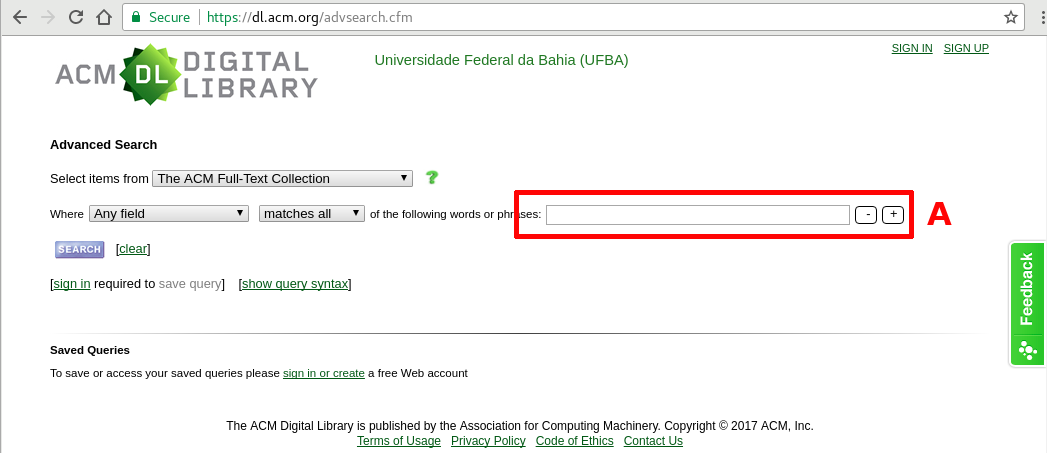
\includegraphics[scale=0.4]{imagens/advanced-search-acm.png}}
  \caption{Captura de tela da busca avançada da base ACM com destaque para (A) campo de entrada da string de busca.}
  \label{advanced-search-acm}
\end{figure}

\begin{figure}[h]
  \center
  \frame{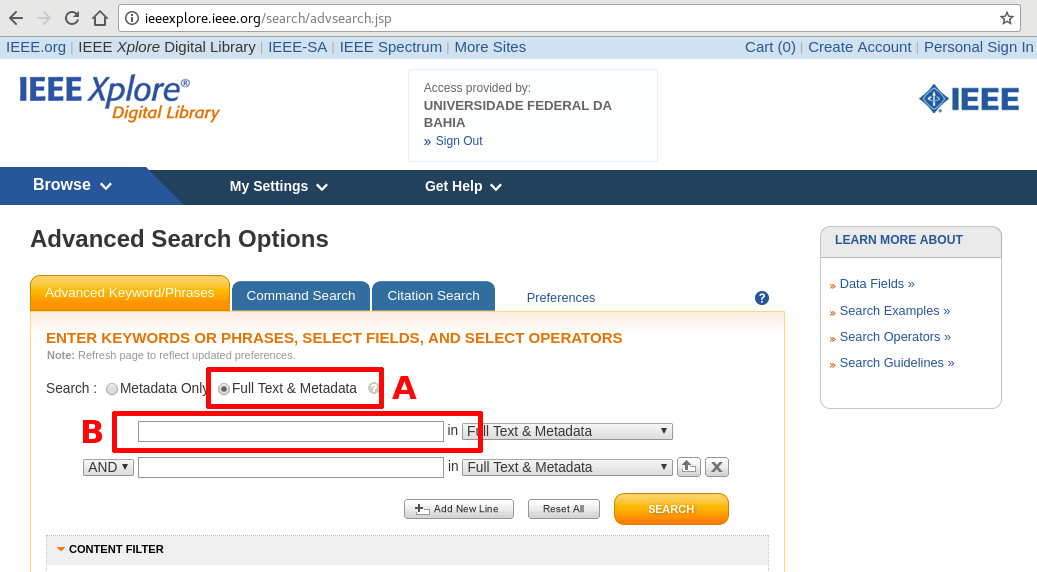
\includegraphics[scale=0.4]{imagens/advanced-search-ieee.png}}
  \caption{Captura de tela da busca avançada da base IEEE com destaque para (A) opção de busca completa e (B) campo de entrada da string de busca.}
  \label{advanced-search-ieee}
\end{figure}

O resultado da busca final de cada projeto em cada base deve ser exportado e
copiado localmente em formato BibTeX, e ambas as bases exportam os resultados
neste formato. Os resultados finais da busca de todos os projetos serão combinados
e agregados num resultado único, sem duplicação de resultados, contendo os
metadados de todos os artigos, sem repetição.

Este resultado final, além de eliminar a duplicação de resultados, será a base
para a definição de uma identificação única para cada artigo encontrado; esta
identificação será utilizada nos próximos passos para relacionar os projetos
aos artigos através das menções encontradas. Por fim, será feito o download de cada
artigo em formato pdf para inspeção manual na etapa seguinte.

\subsection{Passo 2: Triagem}

No passo 2, uma triagem de artigos relevantes é realizada por meio 
de inspeção manual de cada artigo associado aos projetos de software acadêmico
que foi identificado no passo 1.
O critério de inclusão para a seleção de artigos relevantes é a simples
ocorrência do nome do projeto de software acadêmico no artigo.
%
Entre os resultados de cada projeto,
um artigo deverá ser identificado como
relevante para o projeto caso o critério de inclusão seja satisfeito durante a
inspeção manual do artigo.

Ao final deste passo, teremos, para cada projeto
de software acadêmico, um conjunto de artigos identificados como relevantes que fazem
menção ao nome do projeto.

\subsection{Passo 3: Keywording}

Neste passo será criado um esquema de codificação para caracterização das
menções. O esquema é criado a partir da \textit{identificação do contexto} em que os
projetos são mencionados. Para cada menção, toma-se nota sobre como o projeto de
software é mencionado no artigo.

As notas são comentários livres descrevendo as menções encontradas no artigo
sobre um determinado software.
Um artigo científico pode mencionar um software
diversas vezes, de diversas formas, desde uma simples menção nos trabalhos
relacionados até uma grande contribuição ao software.

O conjunto final de todas as anotações é analisado
para definição do esquema de codificação para caracterização das menções. 
Este esquema deve ser construído com o objetivo de agrupar e caracterizar os tipos
de menção encontrados para cada projeto de software em termos da contribuição
que a menção traz ao ecossistema de software daquele projeto acadêmico.

\subsection{Passo 4: Extração}

Neste último passo da revisão de literatura, utiliza-se o esquema de codificação
para caracterização de menções criado no Passo 3 (Keywording) para classificar as
menções de cada projeto de software encontradas nos artigos relevantes
selecionados no Passo 2 (Triagem).

Para cada artigo que menciona um certo projeto de software será associada uma
informação que indique o tipo de menção entre as opções do esquema de
codificação para caracterização das menções. Os artigos selecionados no estudo
anterior (capítulo~\ref{estudo1}) devem também ser adicionados aqui, já que
sabe-se que eles mencionam os projetos de software acadêmico estudados.

Ao final da revisão de literatura, teremos, para cada projeto de software, um
conjunto de artigos relevantes mencionando o software, com indicação do tipo de menção
através do esquema de codificação para caracterização de menções elaboradas no Passo 3 (Keywording).

% }}}

\section{Preparação} \label{estudo2:preparacao} % {{{

Nesta seção apresentamos a preparação do estudo para a realização da coleta de
dados, incluindo a definição de arquivos e formatos de armazenamento, bem como
a implementação de scripts para coleta, análise e transformação.
A Figura \ref{estudo2-fluxograma} apresenta uma visão geral da solução adotada
e da relação entre os passos da revisão de literatura, detalhados a seguir.

\begin{figure}[h]
  \center
  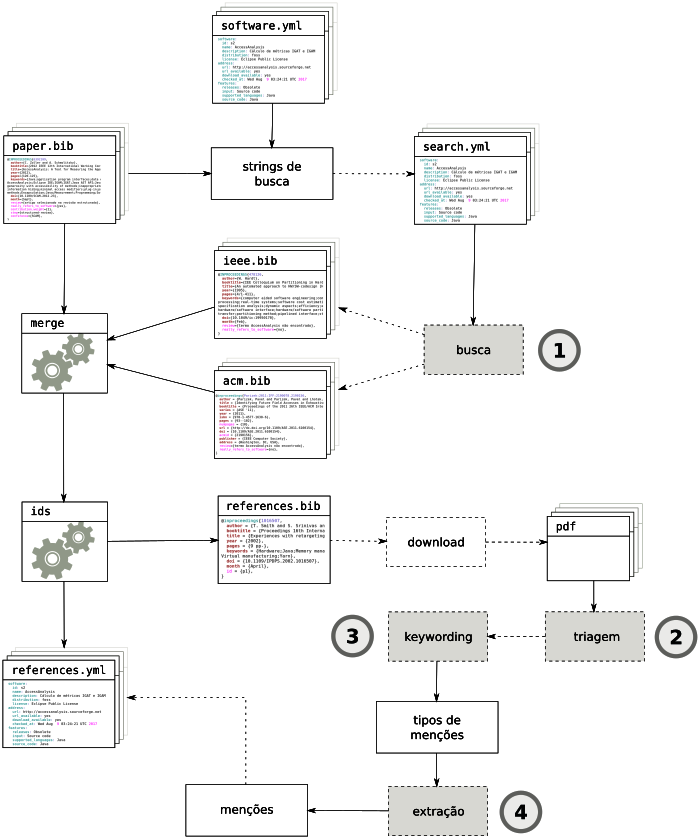
\includegraphics[scale=0.35]{imagens/estudo2-fluxograma.png}
  \caption{Fluxo de coleta, análise e transformação dos dados.}
  \label{estudo2-fluxograma}
\end{figure}

Seguindo o planejamento descrito na seção \ref{estudo2:planejamento},
no passo de busca, 
criamos as strings de busca e as registramos nos arquivos \texttt{search.yml} de cada
projeto. Este arquivo também registra o número de resultados e a data de
execução da busca. A Listagem \ref{search-yml} apresenta um exemplo deste
arquivo com campos utilizados para registrar os resultados da busca.

\begin{lstlisting}[
caption={Arquivo search.yml.},
label={search-yml},
frame=single,
numbers=left
]
  acm:
    string:
    searched_at:
    results:
  ieee:
    string:
    searched_at:
    results:
\end{lstlisting}

Para cada projeto de software acadêmico, outros dois arquivos,
\texttt{acm.bib} e \texttt{ieee.bib}, serão criados para armazenar os dados dos artigos
retornados pela busca. Estes dados, de todos os projetos, serão agregados no
arquivo \texttt{documents/references.bib} e identificados com
o campo \texttt{id} recebendo valores no formato \texttt{p + NÚMERO},
exemplo, \texttt{p1}, \texttt{p2}, \texttt{p3}, ..., \texttt{p806}.

Foi implementado o script \texttt{bin/ids} para automatizar a
definição deste novo campo para cada artigo; ele recebe como entrada um arquivo
no formato BibTeX e gera sequencialmente o campo \texttt{id} para cada item.

Na preparação para a Triagem,
definimos a estrutura do arquivo \texttt{references.yml} onde será registrada a
informação dos artigos relevantes para cada projeto. A Listagem
\ref{references-yml} apresenta um exemplo deste arquivo e de sua estrutura.

\begin{lstlisting}[
caption={Arquivo references.yml.},
label={references-yml},
frame=single,
numbers=left
]
  p1:
    review:
    is_software_mentioned:
  p2:
    review:
    is_software_mentioned:
  p3:
    review:
    is_software_mentioned:
\end{lstlisting}

Em paralelo a definição deste arquivo, implementamos um mecanismo de templates,
por meio dos scripts \texttt{bin/cache} e \texttt{bin/render}, para criação
automática desses arquivos para cada projeto. 
Este mecanismo é apresentado em resumo na Figura
\ref{template-fluxograma}.
O mecanismo de templates será
utilizado em outros pontos de estudo para automatizar e produzir documentos a
partir dos dados coletados.

\begin{figure}[h]
  \center
  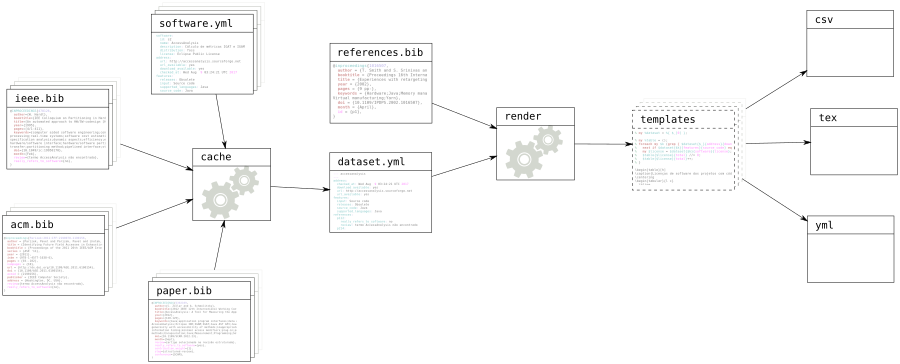
\includegraphics[scale=0.3]{imagens/template-fluxograma.png}
  \caption{Mecanismo de template para transformar dados em documentos para visualização e análise.}
  \label{template-fluxograma}
\end{figure}

O script \texttt{bin/cache} cria o arquivo \texttt{cache/dataset.yml} ao
agregar todos os dados coletados de todos os projetos a partir dos arquivos
\texttt{software.yml}, \texttt{acm.bib}, \texttt{ieee.bib}, \texttt{paper.bib},
\texttt{references.yml} e \texttt{search.yml}.
O script \texttt{bin/render} lê este arquivo \texttt{cache/dataset.yml},
carrega os dados em memória e passa estes dados como parâmetro para os arquivos
templates.

Para apoiar o passo de Keywording, 
adicionamos aos arquivos \texttt{references.yml} um novo campo para coletar o
tipo de menção feita em cada artigo aos projetos, \texttt{mention\_type}. 
Este campo assume um dos valores do esquema de classificação de menções 
a ser criado durante a execução desse passo.

Finalmente, para apoiar o passo de extração, 
implementamos arquivos de template para representar os dados coletados em
outros formatos para visualização e análise, incluindo documentos em formatos
CSV, Markdown e \LaTeX. Alguns destes documentos são incluídos automaticamente
neste texto.

% }}}

\section{Coleta de Dados} \label{estudo2:coleta} % {{{

Seguindo o planejamento e preparação descritos nas seções
\ref{estudo2:planejamento} e \ref{estudo2:preparacao}, iniciamos a atividade de coleta de
dados através da revisão de literatura.
A Figura \ref{estudo2-revisao-literatura} apresenta um resumo dos passos da revisão da literatura
realizada nas bases ACM e IEEE.

\begin{figure}[h]
  \center
  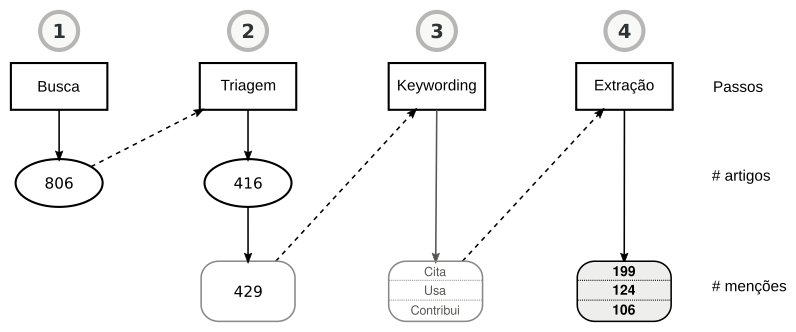
\includegraphics[scale=0.35]{imagens/estudo2-revisao-literatura.png}
  \caption{Passos da revisão de literatura realizada nas bases ACM e IEEE.}
  \label{estudo2-revisao-literatura}
\end{figure}

A busca de todos os projetos retornou \SearchCount \ resultados,
\SearchACMCount \ na base ACM e \SearchIEEECount \ na base IEEE.
Estes resultados incluem duplicação de artigos, ou seja,
um mesmo artigo encontrado nas duas bases, ou, um mesmo artigo
encontrado em relação a mais de um projeto, dentre o resultado total.

Ao remover as duplicidades temos um conjunto de \SearchUniqueCount \ artigos
únicos. A Tabela \ref{search-table} apresenta o total de resultados para cada
um dos projetos pesquisados; a coluna {\bf Total} inclui os artigos do arquivo
\texttt{paper.bib} e apresenta apenas resultados únicos.

\begin{longtable}{ l c c c | l c c c }
\caption{Número de resultados obtidos na busca de cada projeto de software.}
\label{search-table} \\
  \hline
  \hhline{ l c c c | l c c c |}
  \endfirsthead
  \hhline{ l c c c | l c c c |}
  \hline
   \multirow{2}{*}{\textbf{ID}} & \multicolumn{2}{c}{{\bf Busca}} & \multirow{2}{*}{\textbf{Total}} & \multirow{2}{*}{\textbf{ID}} & \multicolumn{2}{c}{{\bf Busca}} & \multirow{2}{*}{\textbf{Total}} \\
   & \textbf{ACM} & \textbf{IEEE} & & & \textbf{ACM} & \textbf{IEEE} & \\
  \hline
  \hhline{ l c c c | l c c c |}
  \endhead
  \hhline{----|----}
  \multicolumn{8}{c}{continua na próxima página} \\
  \hhline{----|----} \endfoot
  \hhline{----|----} \endlastfoot
   \multirow{2}{*}{\textbf{ID}} & \multicolumn{2}{c}{{\bf Busca}} & \multirow{2}{*}{\textbf{Total}} & \multirow{2}{*}{\textbf{ID}} & \multicolumn{2}{c}{{\bf Busca}} & \multirow{2}{*}{\textbf{Total}} \\
   & \textbf{ACM} & \textbf{IEEE} & & & \textbf{ACM} & \textbf{IEEE} & \\
  \hline
\texttt{s1} & 11 & 26 & 38 & \texttt{s32} & 19 & 18 & 32 \\
\texttt{s2} & 5 & 3 & 8 & \texttt{s33} & 3 & 3 & 5 \\
\texttt{s3} & 10 & 6 & 15 & \texttt{s34} & 1 & 3 & 4 \\
\texttt{s4} & 4 & 6 & 9 & \texttt{s35} & 2 & 1 & 2 \\
\texttt{s5} & 4 & 3 & 6 & \texttt{s36} & 17 & 20 & 34 \\
\texttt{s6} & 6 & 2 & 7 & \texttt{s37} & 2 & 5 & 7 \\
\texttt{s7} & 16 & 9 & 25 & \texttt{s38} & 29 & 20 & 42 \\
\texttt{s8} & 7 & 7 & 13 & \texttt{s39} & 3 & 10 & 11 \\
\texttt{s9} & 4 & 4 & 8 & \texttt{s40} & 3 & 8 & 11 \\
\texttt{s10} & 12 & 4 & 14 & \texttt{s41} & - & - & 1 \\
\texttt{s11} & 2 & 2 & 3 & \texttt{s42} & 1 & 4 & 5 \\
\texttt{s12} & 6 & 1 & 6 & \texttt{s43} & - & 2 & 2 \\
\texttt{s13} & 6 & 3 & 9 & \texttt{s44} & 3 & 1 & 3 \\
\texttt{s14} & 1 & 1 & 2 & \texttt{s45} & 5 & 10 & 14 \\
\texttt{s15} & 15 & 4 & 16 & \texttt{s46} & 16 & 12 & 24 \\
\texttt{s17} & - & 1 & 1 & \texttt{s47} & 6 & 7 & 13 \\
\texttt{s16} & 1 & 4 & 5 & \texttt{s48} & 3 & 2 & 4 \\
\texttt{s18} & 23 & 24 & 47 & \texttt{s49} & 1 & 4 & 5 \\
\texttt{s19} & 20 & 30 & 45 & \texttt{s50} & 1 & 1 & 2 \\
\texttt{s20} & 7 & 3 & 10 & \texttt{s51} & 2 & 5 & 7 \\
\texttt{s21} & 1 & 3 & 3 & \texttt{s52} & 9 & 34 & 41 \\
\texttt{s22} & 4 & 4 & 5 & \texttt{s53} & 10 & 5 & 13 \\
\texttt{s23} & 2 & 11 & 12 & \texttt{s54} & 2 & 2 & 4 \\
\texttt{s24} & - & - & 1 & \texttt{s55} & 3 & 8 & 12 \\
\texttt{s25} & 20 & 17 & 34 & \texttt{s56} & 23 & 21 & 38 \\
\texttt{s26} & 5 & 2 & 7 & \texttt{s57} & 4 & 6 & 8 \\
\texttt{s27} & 2 & 4 & 5 & \texttt{s58} & 8 & 4 & 11 \\
\texttt{s28} & 26 & 24 & 50 & \texttt{s59} & 25 & 12 & 36 \\
\texttt{s29} & 11 & 5 & 15 & \texttt{s60} & - & 7 & 7 \\
\texttt{s30} & 4 & 9 & 10 & \texttt{{\bf Média}} & {\bf 7.3} & {\bf 7.7} & {\bf 13.8} \\
\texttt{s31} & 2 & 2 & 3 & \texttt{{\bf Total}} & {\bf 438} & {\bf 459} & {\bf 830} \\
\end{longtable}


Durante a triagem, 
os \SearchUniqueCount \ artigos foram inspecionados em busca de menções aos
projetos de software. Encontramos \ScreeningCount \ menções entre
\ScreeningUniqueCount \ artigos.
Alguns projetos de software possuem nomes comuns que foram encontrados nos
artigos mas que não faziam referencia ao software; em alguns casos, os nomes
apareciam em fórmulas matemáticas ou como parte do texto em contextos não
relacionados ao projeto de software acadêmico.

A Figura \ref{screenshot-paper-p148-2ls} apresenta um destes casos. O nome do
projeto \texttt{s1} (2LS) foi encontrado no artigo \texttt{p148} (Statistical
Design Framework of Submicron Flip-Flop Circuits Considering Process
Variations) em contexto sem relação alguma com o projeto em sí.

Ao final da triagem, temos, para cada projeto, um conjunto de artigos que, de
fato, mencionam o software acadêmico, mas sem caracterizar o tipo de menção.

\begin{figure}[h]
  \center
  \frame{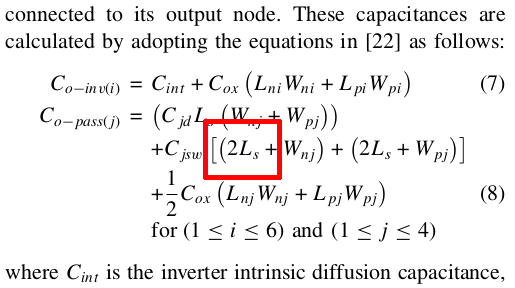
\includegraphics[scale=0.45]{imagens/screenshot-paper-p148-2ls.png}}
  \caption{Exemplo de ocorrência do nome do projeto de software em fórmula matemática.}
  \label{screenshot-paper-p148-2ls}
\end{figure}

Na execução do passo de Keywording, 
a anotação de cada uma das \ScreeningCount \ menções foram analisadas e o
esquema para caracterização foi criado, com três valores distintos que
indicam o nível de contribuição da menção ao ecossistema de software do projeto,
conforme Tabela \ref{esquema-de-mencao}.

\begin{table}[h]
\caption{Esquema para classificação de menções aos projetos software acadêmico.}
\centering
\begin{tabular}{ l p{10cm} }
  \hline
  Tipo de menção           & Explicação \\
  \hline
  Cita      & É o mesmo artigo selecionado em \texttt{paper.bib} (artigo com ``mesmo'' conteúdo publicado na ``mesma'' época); Descreve o software; Menciona o software numa tabela com outros, classifica, cita como exemplo; Menciona em trabalhos relacionados ou em trabalhos futuros. \\
  Usa       & Avalia ou caracteriza o software; Usa para coleta ou análise de dados; Usa como objeto de estudo; Usa o software como parte de uma solução, implementação, etc; Cria um software derivado sem disponibilizar as contribuições. \\
  Contribui & Contribuição inicial publicando o software; Refatora o software; Abre o código de um software que antes era código fechado; Contribuição em código fonte; Extende o software; Integra o software a outros sistemas, formatos de entrada/saída ou APIs; Implementa parte do software em outro projeto e compara resultados. \\
  \hline
\end{tabular}
\label{esquema-de-mencao}
\end{table}

A partir do esquema para caracterização das menções, coletamos os valores
assumindo um dos valores da Tabela \ref{esquema-de-mencao}. Encontramos
\CiteCount \ menções do tipo Cita, \UseCount \ menções do tipo Usa e
\ContributeCount \ menções do tipo Contribui. Estes dados são
apresentados em resumo na Tabela \ref{mentions-table}.

\begin{longtable}{ l c c c c | l c c c c }
\caption{Número de menções por tipo para cada projeto.}
\label{mentions-table} \\
  \hline
  \hhline{ l c c c c | l c c c c |}
  \endfirsthead
  \hhline{ l c c c c | l c c c c |}
  \hline
   \multirow{2}{*}{\textbf{ID}} & \multicolumn{3}{c}{{\bf Menções}} & \multirow{2}{*}{\textbf{Total}} & \multirow{2}{*}{\textbf{ID}} & \multicolumn{3}{c}{{\bf Menções}} & \multirow{2}{*}{\textbf{Total}} \\
   & \textbf{Cita} & \textbf{Usa} & \textbf{Contribui} & & & \textbf{Cita} & \textbf{Usa} & \textbf{Contribui} & \\
  \hline
  \hhline{ l c c c c | l c c c c |}
  \endhead
  \hhline{-----|-----}
  \multicolumn{10}{c}{continua na próxima página} \\
  \hhline{-----|-----} \endfoot
  \hhline{-----|-----} \endlastfoot
   \multirow{2}{*}{\textbf{ID}} & \multicolumn{3}{c}{{\bf Menções}} & \multirow{2}{*}{\textbf{Total}} & \multirow{2}{*}{\textbf{ID}} & \multicolumn{3}{c}{{\bf Menções}} & \multirow{2}{*}{\textbf{Total}} \\
   & \textbf{Cita} & \textbf{Usa} & \textbf{Contribui} & & & \textbf{Cita} & \textbf{Usa} & \textbf{Contribui} & \\
  \hline
\texttt{s1} & - & - & 1 & 1 & \texttt{s32} & 8 & - & 6 & 14 \\
\texttt{s2} & 1 & - & 1 & 2 & \texttt{s33} & 2 & 2 & 1 & 5 \\
\texttt{s3} & 3 & - & 1 & 4 & \texttt{s34} & 1 & - & 1 & 2 \\
\texttt{s4} & 4 & 3 & 2 & 9 & \texttt{s35} & - & - & 1 & 1 \\
\texttt{s5} & 2 & - & 3 & 5 & \texttt{s36} & 1 & - & 1 & 2 \\
\texttt{s6} & 4 & - & 1 & 5 & \texttt{s37} & 3 & 1 & 3 & 7 \\
\texttt{s7} & 9 & - & 1 & 10 & \texttt{s38} & 17 & - & 1 & 18 \\
\texttt{s8} & 3 & 1 & 2 & 6 & \texttt{s39} & 1 & - & 1 & 2 \\
\texttt{s9} & - & - & 5 & 5 & \texttt{s40} & 1 & 5 & 3 & 9 \\
\texttt{s10} & 1 & 2 & 2 & 5 & \texttt{s41} & - & - & 1 & 1 \\
\texttt{s11} & 2 & - & 1 & 3 & \texttt{s42} & - & - & 1 & 1 \\
\texttt{s12} & 1 & - & 1 & 2 & \texttt{s43} & - & - & 2 & 2 \\
\texttt{s13} & - & - & 1 & 1 & \texttt{s44} & 1 & - & 1 & 2 \\
\texttt{s14} & 1 & - & 1 & 2 & \texttt{s45} & - & - & 2 & 2 \\
\texttt{s15} & 4 & - & 1 & 5 & \texttt{s46} & 9 & 3 & 1 & 13 \\
\texttt{s17} & - & - & 1 & 1 & \texttt{s47} & - & - & 1 & 1 \\
\texttt{s16} & 1 & 1 & 2 & 4 & \texttt{s48} & 1 & - & 1 & 2 \\
\texttt{s18} & - & 1 & 1 & 2 & \texttt{s49} & 1 & 2 & 2 & 5 \\
\texttt{s19} & 14 & 18 & 8 & 40 & \texttt{s50} & - & - & 1 & 1 \\
\texttt{s20} & - & - & 1 & 1 & \texttt{s51} & 1 & 2 & 1 & 4 \\
\texttt{s21} & - & - & 1 & 1 & \texttt{s52} & 14 & 23 & 3 & 40 \\
\texttt{s22} & 2 & - & 1 & 3 & \texttt{s53} & 1 & 2 & 1 & 4 \\
\texttt{s23} & 3 & 2 & 3 & 8 & \texttt{s54} & 1 & 1 & 1 & 3 \\
\texttt{s24} & - & - & 1 & 1 & \texttt{s55} & - & - & 1 & 1 \\
\texttt{s25} & 5 & 10 & 4 & 19 & \texttt{s56} & 15 & 5 & 1 & 21 \\
\texttt{s26} & 3 & 2 & 2 & 7 & \texttt{s57} & 4 & - & 1 & 5 \\
\texttt{s27} & - & 2 & 1 & 3 & \texttt{s58} & 5 & 5 & 1 & 11 \\
\texttt{s28} & 22 & 14 & 4 & 40 & \texttt{s59} & 16 & 10 & 7 & 33 \\
\texttt{s29} & 5 & 1 & 1 & 7 & \texttt{s60} & 4 & - & 1 & 5 \\
\texttt{s30} & 2 & 5 & 1 & 8 & \texttt{{\bf Média}} & {\bf 3.3} & {\bf 2.1} & {\bf 1.8} & {\bf 7.2} \\
\texttt{s31} & - & 1 & 1 & 2 & \texttt{{\bf Total}} & {\bf 199} & {\bf 124} & {\bf 106} & {\bf 429} \\
\end{longtable}


É importante lembrar que as menções do tipo Contribui incluem os artigos
selecionados no arquivo \texttt{paper.bib}, independente de terem sido
encontrados na busca das bases ACM e IEEE, mas ao discutir e interpretar os
dados saberemos distinguir e separar estes dois grupos quando necessário.

% }}}

\section{Análise dos Dados} \label{estudo2:analise} % {{{

A análise de dados foi realizada considerando
dados de \SoftwareCount \ projetos desenvolvidos e publicados na literatura
acadêmica de Engenharia de Software, informações sobre diversas formas de
menção ao nome destes projetos, e \ScreeningUniqueCount \ artigos distintos
encontrados nas bases ACM e IEEE mencionando estes projetos.

A busca nas bases ACM e IEEE retornou uma média de \SearchUniqueMean \ artigos
por projeto de software acadêmico. 
Os projetos \texttt{s24} (GUIZMO) e \texttt{s41} (protopurity)
não foram encontrados em nenhuma das bases.
Os projetos \texttt{s17} (e-munity), \texttt{s43} (PtYasm) e \texttt{s60} (XOgastan)
não foram encontrados na base ACM.

Entre os projetos com resultados acima da média, 
a maior parte está disponível para download, 
sendo 11 com acesso e 7 sem acesso.  
Do mesmo modo, entre os projetos com resultados abaixo da média, 
a maior parte, 25 projetos, está disponível para download, 
e 16 não estão disponíveis para download.

Na triagem, observou-se que:

\begin{itemize}
  \item Entre os resultados da busca, apenas 51\% dos artigos são relevantes e
    fazem menção aos projetos, com uma média de \ScreeningUniqueMean \ artigos
    por projeto e \ScreeningMean \ menções por projeto;
  \item Entre os projetos com menções acima da média, 9 estão disponíveis para
    download e 6 não estão disponíveis. Entre os projetos com menções abaixo da
    média, 25 possuem download disponível e 20 não estão disponíveis.
\end{itemize}

Durante o Keywording notamos que os três tipos de menção -- Cita, Usa e
Contribui -- que emergiram das avaliações a respeito do contexto em que as
menções ocorrem, possuem a natureza de uma escala de valores, sendo este valor
uma representação da contribuição que cada menção causa no software acadêmico
ou no seu ecossistema, sendo o tipo Cita o primeiro valor de menor peso e o
tipo Contribui com o maior peso de contribuição ao software e ao seu
ecossistema.

Durante a extração, observou-se que, 
entre os \SoftwareCount \ projetos, \SoftwareNotMentionedCount \ projetos
(\texttt{s1}, \texttt{s13}, \texttt{s17}, \texttt{s20}, \texttt{s21}, \texttt{s24}, \texttt{s35}, \texttt{s41}, \texttt{s42}, \texttt{s43}, \texttt{s47}, \texttt{s50}, \texttt{s55}, \texttt{s61}, \texttt{s62}, \texttt{s63}, \texttt{s65}, \texttt{s66}, \texttt{s68}
) não foram encontrados em menções
após a publicação inicial, sendo a única publicação aquela localizada no
arquivo \texttt{paper.bib}, referente a seleção do software no estudo
apresentado no Capítulo \ref{estudo1}.
%
Os demais \MentionsStudyDois \ projetos são mencionados em publicações nas
bases ACM e IEEE. Deste grupo, apenas \ContributeStudyDoisSoftware \ projetos
(\texttt{s10}, \texttt{s19}, \texttt{s23}, \texttt{s25}, \texttt{s26}, \texttt{s28}, \texttt{s32}, \texttt{s37}, \texttt{s4}, \texttt{s40}, \texttt{s45}, \texttt{s49}, \texttt{s5}, \texttt{s52}, \texttt{s59}, \texttt{s67}, \texttt{s8}, \texttt{s9}
) recebem contribuições através de
\ContributeStudyDoisCount \ menções.

A Figura \ref{mentions-timeline} apresenta uma visualização da linha do tempo
de cada software acadêmico em relação a menções encontradas nas bases ACM e IEEE.

\begin{figure}[h]
  \center
  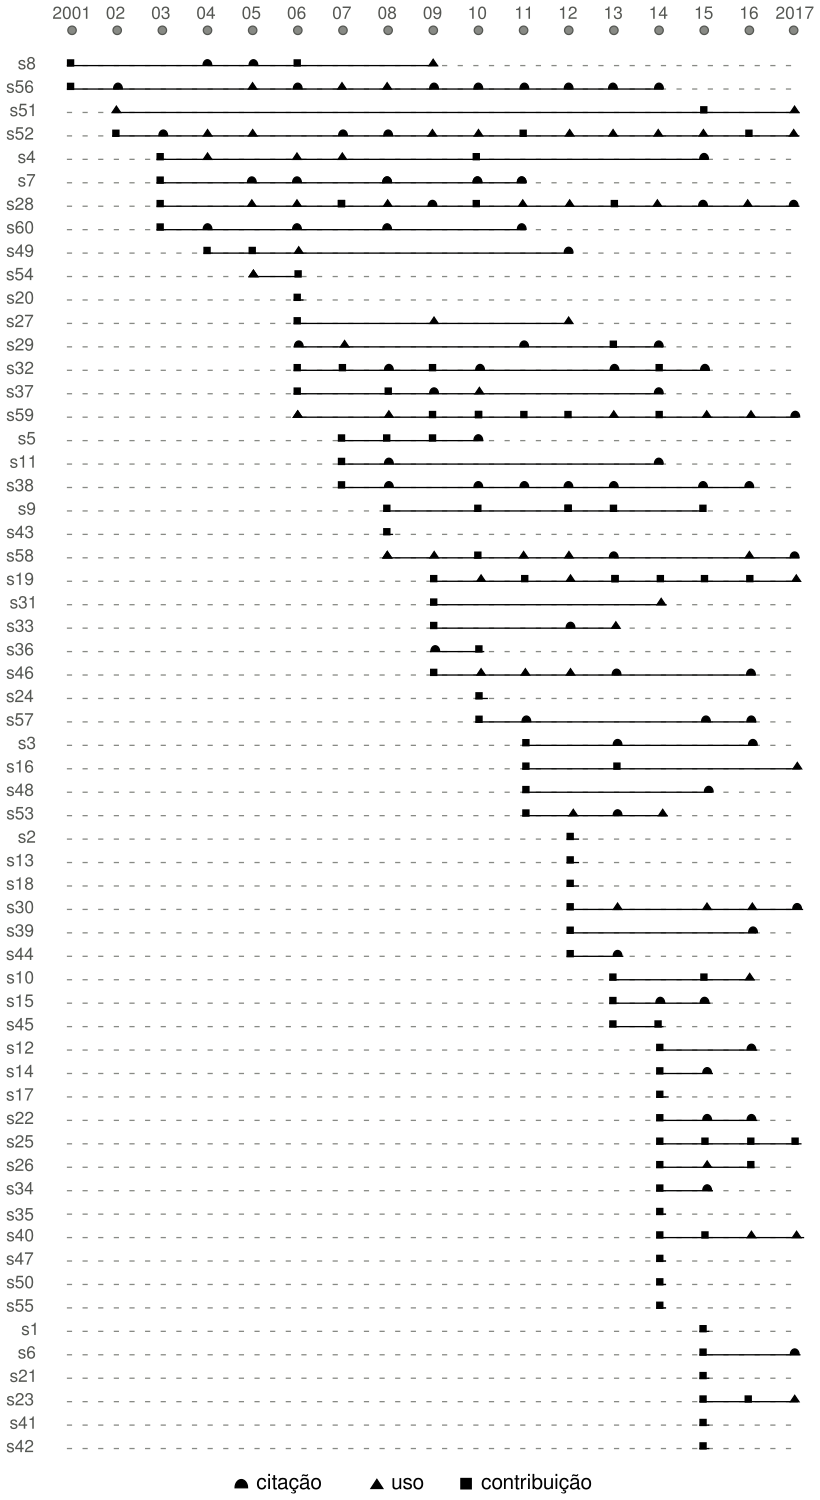
\includegraphics[scale=0.6]{imagens/mentions-timeline.png}
  \caption{Linha do tempo de menções (uso e contribuição) aos projetos nas bases ACM e IEEE.}
  \label{mentions-timeline}
\end{figure}

% }}}

\section{Interpretação dos Resultados} \label{estudo2:interpretacao} % {{{

\subsection{Q1 - \EstudoDoisQuestaoUm}

Os \SoftwareCount \ projetos de software acadêmico de análise estática
publicados nas conferências ASE e SCAM são mencionados \ScreeningCount \ vezes
em \ScreeningUniqueCount \ artigos distintos, estas menções foram encontradas
em buscas nas bases ACM e IEEE realizadas entre os meses de Julho e Agosto de
2017.

Entre todas as menções emergiu três tipos distintos em relação ao nível de
contribuição ao ecossistema dos projetos, Cita, Usa e Contribui. A maior parte
das menções encontradas é do tipo Cita (\CiteCount \ menções), em seguida
o tipo de menção Usa com \UseCount \ ocorrências, e por fim, com menor número,
o tipo de menção Contribui com \ContributeCount \ ocorrências.

\subsection{Q2 - \EstudoDoisQuestaoDois}

Encontramos \UseCount \ menções usando os projetos como apoio metodológico para
coleta ou análise de dados, como objeto de estudo, ou como ponto de partida
para implementação de outras soluções de pesquisa.

Estas menções do tipo Uso estão associadas a 26 dos \SoftwareCount \ projetos
de software, indicando que menos da metade dos projetos de software acadêmico
de análise estática publicados nas conferências ASE e SCAM são utilizados em
pesquisas nas bases ACM e IEEE.

\subsection{Q3 - \EstudoDoisQuestaoTres}

Encontramos \ContributeCount \ menções contribuindo com os projetos, este total
inclui os artigos publicando os projetos de software pela primeira vez, ou
seja, inclui os artigos que deram origem ao conjunto de \SoftwareCount \
projetos de software registrados nos arquivos \texttt{paper.bib}.

Ao analisar apenas contribuições posteriores a publicação inicial
do projeto, ou seja, artigos e estudos contribuindo com código
fonte aos projetos após a sua publicação inicial, encontramos
\ContributeStudyDoisCount \ menções a um conjunto de
\ContributeStudyDoisSoftware \ projetos de software.

Ou seja, apenas 28\% dos projetos (\texttt{s10}, \texttt{s19}, \texttt{s23}, \texttt{s25}, \texttt{s26}, \texttt{s28}, \texttt{s32}, \texttt{s37}, \texttt{s4}, \texttt{s40}, \texttt{s45}, \texttt{s49}, \texttt{s5}, \texttt{s52}, \texttt{s59}, \texttt{s67}, \texttt{s8}, \texttt{s9}
)
recebem contribuição em código fonte de estudos após a publicação inicial, ao
menos entre estudos encontrados nas bases ACM e IEEE.

% }}}

\section{Ameaças à Validade}  \label{estudo2:ameacas} % {{{

A inspeção manual dos artigos na revisão de literatura em busca de caracterizar
as menções e seus tipos foi realizada apenas pelo autor desta dissertação, isto
pode levar a inconsistência na interpretação das menções em relação aos projetos
investigados, uma vez que a inspeção é realizada num processo estritamente
subjetivo, esta ameaça não foi tratada.

A busca realizada apenas nas bases da ACM e IEEE pode ter deixado fora dos
resultados possíveis artigos mencionando os projetos investigados, uma vez que
é possível que existam publicações não indexadas por estas bases, Apesar disso,
estas duas bases possuem grande relevância para a área de Engenharia de
Software, de forma que esta ameaça não prejudica as conclusões do estudo, uma
vez que todas as conclusões estão estreitamente associadas a este recorte e não
sugerimos serem generalizadas.

É possível que a falta de contribuição aos projetos seja um reflexo da
relevância do estudo onde foram publicados, ou seja, projetos publicados em
artigos com pouca relevância, com pouca visibilidade, pode, eventualmente,
atrair pouca atenção, consequentemente receber pouca contribuição. No entanto,
a relevância do software não está necessariamente associada a relevância do
estudo, é possível que projetos de software extremamente úteis e relevantes
para a comunidade científica tenham sido publicados em artigos com pouca ou
nenhuma relevância. Dessa forma esta ameaça não impacta negativamente as nossas
conclusões, uma vez que estamos interessados em capturar quanta colaboração há
entre os projetos, do ponto de vista de sua utilidade para o corpo científico
como um todo.

% }}}

\section{Conclusões} \label{estudo2:conclusoes} % {{{

Este estudo inspecionou \SearchUniqueCount \ artigos encontrados nas bases ACM
e IEEE através de busca avançada, usando características de \SoftwareCount \
projetos de software acadêmico de análise estática. Durante a inspeção foram
encontradas \ScreeningCount \ menções dos tipos Cita, Usa ou
Contribui.

Estes tipos emergiram da análise sobre como os projetos são mencionados nos
artigos. Entre todas as menções, \CiteCount \ são do tipo Cita, \UseCount \ Usa
e \ContributeCount \ Contribui. As menções do tipo Contribui incluem os artigos
iniciais que publicaram os projetos pela primeira vez pelos autores originais;
ao excluir estes artigos, encontramos apenas \ContributeStudyDoisCount \ menções
do tipo Contribui.

Este número de menções está relacionado a apenas 28\% do conjunto total de
projetos. Isto indica que não parece haver uma prática de contribuição entre os
pesquisadores em relação a código fonte dos seus projetos de software, ao menos
no contexto de análise estática.

Não encontramos relação entre a disponibilidade de download, forma de
distribuição ou linguagem de programação e o número de menções, entre os
projetos com maior contribuição temos Java, C, Erlang e Rascal.

Acreditamos que o número de menções, seja de Uso ou Contribuição, está
intimamente ligado a relevância prática do projeto e aos atributos de
qualidade, como, usabilidade, portabilidade, facilidade de instalação, entre
outros. No entanto, não investigamos estes atributos neste estudo.

Acreditamos fortemente que manutenibilidade, ou seja, o esforço necessário para
realizar alteraçoes no código fonte de um software, está intrinsicamente
relacionado ao número de contribuições destes projetos. Desta forma, planejamos
um terceiro estudo para investigar este aspecto de qualidade entre os projetos
estudados.

% }}}
